\documentclass[%
landscape,paperwidth=42in,paperheight=48in,%
margin=2cm,
fontscale=0.295
%fontscale=0.29
]{baposter}

\usepackage{environ}

\NewEnviron{headerblock}[2]{\headerbox{#1}{#2}{\BODY}}

\usepackage{marvosym,url,siunitx,paralist}
\usepackage{amsmath,amssymb,booktabs,dsfont,comment,epstopdf,multirow}
\usepackage{etoolbox}
\robustify\bfseries % requires etoolbox
\newcommand{\minitab}[2][l]{\begin{tabular}{#1}#2\end{tabular}}

\usetikzlibrary{intersections,decorations.pathreplacing,fit,calc,positioning,shapes.geometric,matrix}
\pgfdeclarelayer{background}
\pgfsetlayers{background,main}

\newcommand{\vect}[1]{\vec{#1}}
\newcommand{\mus}{\vec{\mu}}
\newcommand{\data}{\mathcal{D}}
\newcommand{\given}{\mid}
\DeclareMathOperator{\sigm}{sigm}
\DeclareMathOperator{\conj}{conj}
\DeclareMathOperator{\fft}{fft}
\DeclareMathOperator{\ifft}{ifft}
\newcommand{\R}{\ensuremath{\mathds{R}}}
\newcommand{\Q}{\ensuremath{\mathds{Q}}}
\newcommand{\N}{\ensuremath{\mathds{N}}}
\newcommand{\E}{\ensuremath{\mathds{E}}}
\newcommand{\F}{\ensuremath{\mathcal{F}}}
\newcommand{\Norm}{\ensuremath{\mathcal{N}}}

\renewcommand*\sfdefault{uop}
\newcommand{\spanA}{2}
\newcommand{\spanB}{2}

%\selectcolormodel{cmyk}

\begin{document}

%\definecolor{ubcblue}{cmyk}{0.392, 0.352, 0.051, 0.267}
\definecolor{ubcblue}{HTML}{002145}
\definecolor{ubcgraya}{HTML}{5E869F}
\definecolor{ubcgrayb}{HTML}{2F5D7C}
\definecolor{ubcgrayc}{HTML}{98B2C3}
\definecolor{ubcgrayd}{HTML}{C3D0DB}
\definecolor{ubcgrayf}{HTML}{B7C9D3}

\newcommand{\alert}[1]{\textbf{\textcolor{ubcblue}{#1}}}
\newcommand{\minisection}[1]{\textcolor{ubcblue}{\large\textbf{%
\tikz \fill[ubcblue] (0,0)-- ++(90:0.25)-- ++(-30:0.25)--cycle; #1}}\\[0.5em]}
\setdefaultleftmargin{1em}{}{}{}{.5em}{.5em}
\setlength{\plitemsep}{4.0pt plus 1.0pt minus 1.0pt}
\setlength{\pltopsep}{8.0pt plus 1.0pt minus 4.0pt}
\setlength{\plpartopsep}{2.0pt plus 1.0pt minus 1.0pt}

\renewcommand*\descriptionlabel[1]{%
\hspace\labelsep\bfseries\textcolor{ubcblue}{#1}}

\sffamily

%\background{
%\begin{tikzpicture}[remember picture,overlay]%
%  %\draw (current page.north west)+(-2em,2em) node[anchor=north west]
%  %{\includegraphics[height=1.1\textheight]{background}};
%  \fill[ubcgray!20!white] (current page.north west) rectangle (current
%  page.south east);
%  \end{tikzpicture}
%}

\newcommand{\inst}[1]{$^{#1}$}

\begin{poster}{
  %grid=false,
  %eyecatcher=false,
  columns=4,
  background=shadetb,
  bgColorOne=white,
  bgColorTwo=white,
  %bgColorTwo=ubcgrayf,
  headershade=plain,
  headershape=roundedright,
  headerColorOne=ubcblue,
  headerColorTwo=ubcblue,
  borderColor=ubcblue,
  boxshade=none,
  textborder=faded,
  headerborder=open,
  headerFontColor=white,
  headerfont=\scshape\Large,
  linewidth=1pt,
  %headerheight=0.135\textheight,
  %colspacing=1.25em
  headerheight=0.165\textwidth,
  colspacing=1.25em
}
%%% Eye Catcher %%%
{
\includegraphics[height=0.1\textwidth]{images/MICCAI2014-mark}
}
%%% Title %%%
{
% Manifold\hspace{0.5ex}Learning\hspace{0.5ex}of\hspace{0.5ex}Brain\hspace{0.5ex}MRIs\\
% by\hspace{0.5ex}Deep\hspace{0.5ex}Learning~~\vspace{0.5em}
Modeling the Variability in Brain Morphology and Lesion Distribution in
Multiple Sclerosis by Deep Learning\vspace{0.5em}
}
%%% Authors %%%
{
%Tom Brosch$^1$ and Roger Tam$^2$, MS/MRI Research Group, UBC,
%Vancouver\\[0.65ex]
%$^1$\texttt{tombr@msmri.medicine.ubc.ca}, $^2$\texttt{roger.tam@ubc.ca}
Tom Brosch\inst{1,4},
Youngjin Yoo\inst{1,4},
David K.B. Li\inst{2,4},
Anthony Traboulsee\inst{3,4}, and
Roger Tam\inst{2,4}\\[0.65ex]
\large \inst{1}Department of Electrical and Computer Engineering, UBC\quad
\inst{2}Department of Radiology, UBC\quad
\inst{3}Division of Neurology, UBC\\[0.65ex]
\inst{4}MS/MRI Research Group, University of British Columbia, Vancouver, Canada
%\\[0.65ex]
}
%%% Logo %%%
{
\begin{tabular}{c}
\\

\includegraphics[height=0.07\textwidth]{images/s4b282c}\\
\addlinespace

\includegraphics[height=0.03\textwidth]{images/msmri_simple}
\end{tabular}
}

%%%%%%%%%%%%%%%%%%%%%%%%%
% Footer
%%%%%%%%%%%%%%%%%%%%%%%%%

% \begin{headerblock}{}{name=footer, column=0, span=4,
% above=bottom,textborder=none, headerborder=none, boxheaderheight=0pt,
% headershape=rectangle}
% \begin{center}
% \Large
%   \Letter\ \texttt{tombr@msmri.medicine.ubc.ca}\quad
%   \Mundus\ \url{http://tbrosch.blogspot.com/}
% \end{center}
% %\includegraphics[width=\textwidth]{images/MICCAI2014-banner}
% \end{headerblock}

\begin{headerblock}{Acknowledgement}{above=bottom, column=0,
span=2,
%boxheaderheight=1.6em,
name=acknowledgement}

This work was supported by the Natural Sciences and Engineering Research Council
of Canada and the Milan and Maureen Ilich Foundation.

\end{headerblock}

% \begin{headerblock}{\normalsize Contact Information}{above=bottom, column=2,
% span=2, above=bottom, boxheaderheight=1.6em, name=contact}
% %\begin{tabular}{@{}c@{\, }ll}
% % \begin{tabular}{@{}cll}
% %   \Letter & \texttt{tombr@msmri.medicine.ubc.ca} \\
% %   \Mundus & \url{http://tbrosch.blogspot.com/}
% % \end{tabular}
% \Letter\ \texttt{tombr@msmri.medicine.ubc.ca}\quad\Mundus{}
% \url{http://tbrosch.blogspot.com/}
% \end{headerblock}

%%%%%%%%%%%%%%%%%%%%%%%%%
% Introduction
%%%%%%%%%%%%%%%%%%%%%%%%%

\begin{headerblock}{Introduction}{row=0, column=0, span=1,
name=introduction}
\begin{compactitem}
  \item Changes in brain morphology and white matter lesions are two hallmarks
  of multiple sclerosis (MS) pathology, but their variability beyond volumetrics is
poorly characterized.
\item To further our understanding of complex MS pathology, we
aim to build a statistical model of brain images that can automatically discover
spatial patterns of variability in brain morphology and lesion distribution.
\item We propose building such a model using a deep belief network (DBN), a
layered network whose parameters can be learned from training images.
%\item Our model consists of a morphology DBN, a\\ lesion DBN, and a joint DBN.
 %that models concurring morphological and lesion patterns.
\end{compactitem}
\end{headerblock}

%%%%%%%%%%%%%%%%%%%%%%%%%
% Contributions
%%%%%%%%%%%%%%%%%%%%%%%%%

\begin{headerblock}{Contributions}{row=0, column=1, span=1, name=contributions}
\begin{compactitem}
%   \item Does not require a prebuilt proximity graph, which is particularly
%   beneficial for modeling lesions, because the sparseness and randomness of MS
%   lesions make defining a suitable distance measure challenging and potentially
%   biasing.

  \item New method for modeling and visualizing the variability in brain
  morphology and lesion distribution of a large set of MRIs of MS patients
  
  \item In contrast to other manifold learning approaches, our method does not
  require a prebuilt proximity graph. This is particularly beneficial for
  modeling lesions, because the sparseness and randomness of MS lesions make
  defining a suitable distance measure challenging and potentially biasing.

% \item Our model can automatically discover the classic patterns of MS
% pathology, as well as more subtle ones.
% \item The parameters computed by our model have strong relationships to MS
% clinical scores.
\end{compactitem}
\end{headerblock}

%%%%%%%%%%%%%%%%%%%%%%%%%
% Overview
%%%%%%%%%%%%%%%%%%%%%%%%%

% \begin{headerblock}{Overview}{row=0, column=1, span=1}
% \begin{compactdesc}
%   \item[Data set:] 474 T1-weighted, T2-weighted, and PD-weighted MRIs of
%   secondary progressive MS patients with a resolution of \num{256x256x50} voxels
%  and a voxel size of \SI{0.937x0.937x3.000}{\milli\meter}
%  \item[Pre-processing:] Brain extraction, intensity normalization, background
%  cropping, lesion segmentation, affine registration to ICBM 152 nonlinear atlas
%  template image
%  \item[Morphology model:] a model that aims to find patterns of morphological changes in deformation
% fields
% \item[Lesion model:] a model that aims to find patterns in the spatial
% distribution of lesions
% \item[Joint model:] a joint model that aims to find concurring deformation and
% lesion distribution patterns
% \end{compactdesc}
% \end{headerblock}

%%%%%%%%%%%%%%%%%%%%%%%
% Method 
%%%%%%%%%%%%%%%%%%%%%%%
\begin{headerblock}{Method}{below=introduction, column=0, span=2,
name=method,above=acknowledgement}
\begin{compactdesc}
  \item[Data set:] 474 T1-weighted, T2-weighted, and PD-weighted MRIs of
  secondary progressive MS patients with a resolution of \num{256x256x50} voxels
 and a voxel size of \SI{0.937x0.937x3.000}{\milli\meter}
 \item[Pre-processing:] Brain extraction, intensity normalization, background
 cropping, lesion segmentation, affine registration to the ICBM 152 nonlinear
 atlas template image followed by nonlinear registration (FSL FNIRT) to generate the
 displacement fields
 
%  \item[Morphology DBN:] a model that aims to find patterns of morphological
%  changes in deformation fields
% \item[Lesion DBN:] a model that aims to find patterns in the spatial
% distribution of lesions
% \item[Joint DBN:] a joint model that aims to find concurring deformation and
% lesion distribution patterns
\end{compactdesc}
\begin{compactitem}

\item Displacement fields $u$ and lesion masks $l$ are assumed to be samples
from the distributions $p(u \mid D_1, D_2)$ and $p(l \mid L_1, L_2)$, which can
be learned from training data.
 
\item Both distributions are modeled by two individual strided convolutional
DBNs with three strided convolutional restricted Boltzmann machine (RBM) layers
and two dense RBM layers.

% \item Due to the omission of pooling layers, inference is invertible in a
% strided convolutional DBN, which allows the visualization of discovered patters
% of variability

\item To discover concurring patterns of morphology and lesion distribution, we
combine the morphology DBN and the lesion DBN to form the joint DBN, which
defines the joint distribution $p(u, l \mid J_1, J_2, J_3, J_4)$.
 
\end{compactitem}
\vspace{2em}
%\begin{center}
%\begin{tikzpicture}[scale=0.75]
\tikzstyle{every node}=[font=\sffamily\small, inner sep=3pt, align=center]
\tikzstyle{every pin}=[align=center,fill=white]
\tikzstyle{dbnlabel}=[font=\sffamily]
         
% Deformation field
        
\node[dbnlabel, rotate=90] at (-1.5,2.25) {Morphology DBN};
        
\begin{scope}[xshift=-20pt,yslant=0.63,xscale=0.4]

\node[transform shape,pin={[pin
distance=8]125:Displacement\\
field $u$}] (field) at (2,2)
{\includegraphics[width=4cm]{figures/deformation2.png}};

% \node[pin={[pin distance=0.6,overlay]93:Displacement\\
% field $u$}] at ($(field.north west)!0.1!(field.north east)$) {};

\end{scope}
         
% 3-channel input

\foreach \x in {0, 10, 20} {
\begin{scope}[xshift=\x pt]
%\ifnum\x=0
%\path
%\else
\draw[fill=white, fill opacity=0.75]
%\fi
  (0,0) coordinate(A\x) -- ++(90:4) coordinate (B\x) -- ++(30:2) coordinate
  (C\x) -- ++(-90:4) -- cycle;
  

% \begin{scope}[xshift=-50pt,yslant=0.63,xscale=0.4]  
% \node[transform shape,inner sep=0pt] at (2,2)
%   {\includegraphics[width=4cm]{deformation2.png}};
% \end{scope}
  
\draw (0,3)
   ++(30:0.25) \ifnum\x=20 coordinate (a1) \else -- +(0:10pt) +(0:0) \fi
-- ++(90:0.5)  \ifnum\x=20 coordinate (b1) \else -- +(0:10pt) +(0:0) \fi
-- ++(30:0.25) \ifnum\x=20 coordinate (c1) \else -- +(0:10pt) +(0:0) \fi
-- ++(-90:0.5) \ifnum\x=20 coordinate (d1) \else -- +(0:10pt) +(0:0) \fi
-- ++(210:0.25);
\end{scope}
}

%\node[below=4pt,xshift=-3pt] at (A0)  {$u_x$};
%\node[below=4pt] at (A10) {$u_y$};
%\node[below=4pt,xshift=3pt] at (A20) {$u_z$};

\node[pin={[pin distance=5pt]260:$u_x$}] at (A0)  {};
\node[pin={[pin distance=5pt]270:$u_y$}] at (A10)  {};
\node[pin={[pin distance=5pt]290:$u_z$}] at (A20)  {};

% Transition

\draw ($(a1)!0.5!(c1)$) ++(55pt,-5pt) coordinate (e1);
\draw (a1) -- (e1);
\draw (b1) -- (e1);
\draw (c1) --node[pin={[pin distance=1cm]40:Strided\\ convolution}] {} (e1);
\draw (d1) -- (e1);

% First layer hidden units

\foreach \x in {80,85,90,95,100,105} {
\begin{scope}[xshift=\x pt,yshift=1.5cm,scale=0.5]
\draw[fill=white, fill opacity=0.75]
  (0,0) coordinate(A\x) -- ++(90:4) coordinate (B\x) -- ++(30:2) coordinate
  (C\x) -- ++(-90:4) coordinate(D\x) -- cycle;
   
\draw (0,2.5)
   ++(30:0.25) \ifnum\x=105 coordinate (a2) \else -- +(0:10pt) +(0:0) \fi
-- ++(90:1)    \ifnum\x=105 coordinate (b2) \else -- +(0:10pt) +(0:0) \fi
-- ++(30:0.5)  \ifnum\x=105 coordinate (c2) \else -- +(0:10pt) +(0:0) \fi
-- ++(-90:1)   \ifnum\x=105 coordinate (d2) \else -- +(0:10pt) +(0:0) \fi
-- ++(210:0.5);
\end{scope}
}

\draw[decorate,decoration={brace,raise=20pt}] (B0|-C0) --node[above=25pt]
{Strided convolutional RBM} (C105|-C0);

\draw[decorate,decoration={brace,raise=4pt,mirror}]
%(A80) --node[below=8pt] {$N = 32$} (A80-|D105);
(A80) --node[below=8pt] {$N = 32$} (A80-|D105);

\draw ($(a2)!0.5!(c2)$) ++(0:38pt) coordinate (e2);
\draw (a2) -- (e2);
\draw (b2) -- (e2);
\draw (c2) -- (e2);
\draw (d2) -- (e2);

% Second layer hidden units

\foreach \x in {145, 150, ..., 175, 180} {
\begin{scope}[xshift=\x pt,yshift=2.25cm,scale=0.25]
\draw[fill=white, fill opacity=0.75]
  (0,0) coordinate(A\x) -- ++(90:4) coordinate (B\x) -- ++(30:2) coordinate
  (C\x) -- ++(-90:4) coordinate(D\x) -- cycle;
\draw (0,1.75)
   ++(30:0.25) \ifnum\x=180 coordinate (a3) \else -- +(0:20pt) +(0:0) \fi
-- ++(90:2)    \ifnum\x=180 coordinate (b3) \else -- +(0:20pt) +(0:0) \fi
-- ++(30:1)    \ifnum\x=180 coordinate (c3) \else -- +(0:20pt) +(0:0) \fi
-- ++(-90:2)   \ifnum\x=180 coordinate (d3) \else -- +(0:20pt) +(0:0) \fi
-- ++(210:1);
\end{scope}
}

\draw[decorate,decoration={brace,raise=4pt,mirror}]
(A145) --node[below=8pt] {$N = 64$} (A145-|D180);

\draw ($(a3)!0.5!(c3)$) ++(0:18pt) coordinate (e3);
\draw (a3) -- (e3);
\draw (b3) -- (e3);
\draw (c3) -- (e3);
\draw (d3) -- (e3);

% Third layer hidden units

\foreach \x in {200, 205, ..., 240} {
\begin{scope}[xshift=\x pt,yshift=2.625cm,scale=0.125]
\draw[fill=white, fill opacity=0.75]
  (0,0) coordinate(A\x) -- ++(90:4) coordinate (B\x) -- ++(30:2) coordinate
  (C\x) -- ++(-90:4) coordinate(D\x) -- cycle;
\end{scope}
}

% Forth layer visible units (dense)

\begin{scope}[xshift=280pt, yshift=2.75cm]
\foreach \x/\y in {0/-2, 1/-1.5, 2/-1, 3/-0.5, 4/0, 5/0.5, 6/1, 7/1.5, 8/2} {
  \node[circle, draw] (v\x) at (0,\y) {};
}
\end{scope}

\draw[shorten >=10pt,shorten <=10pt,dashed] (A240)--(v0.south west);
\draw[shorten >=10pt,shorten <=10pt,dashed] (A240|-C240)--
node[label=120:Vectorize\\ hidden units] {} (v8.north west);

\draw[decorate,decoration={brace,raise=4pt,mirror}]
(A200) --node[below=8pt,fill=white] {$N = 32$} (A200-|D240);

%\node[rotate=90,fill=white,align=center] at(270pt,2.75cm) {Serialize\\ hidden
%units};

% Forth layer hidden units (dense)

\begin{scope}[xshift=320pt, yshift=2.75cm]
\foreach \x/\y in {0/-1, 1/-0.5, 2/0, 3/0.5, 4/1} {
  \node[circle, draw] (h\x) at (0,\y) {};
}
\end{scope}

\foreach \x in {0, ..., 8} {
  \foreach \y in {0, ..., 4} {
    \draw[very thin] (v\x)--(h\y);
  }
}

\draw[decorate,decoration={brace,raise=20pt}] (v8.west|-C0)
--node[above=25pt] {Dense RBM} (h0.east|-C0);

% Fifth layer hidden units (distribution parameters)

\begin{scope}[xshift=360pt, yshift=2.75cm]
\foreach \x/\y in {1/0.25, 2/-0.25} {
  \node[circle, draw, label=0:$D_\x$] (D\x) at (0,\y) {};
}
\end{scope}

\foreach \x in {0, ..., 4} {
  \foreach \y in {1,2} {
    \draw[very thin] (h\x)--(D\y);
  }
}

% \draw[decorate,decoration={brace,raise=22pt}]
% (D1.north-|D1.east) --node[above,sloped] {Deformation\\ parameters}
% (D2.south-|D2.east);

%%%%%%%%%%%%%%%%%%%%%
% Lesion Model
%%%%%%%%%%%%%%%%%%%%%

\begin{scope}[yshift=-6cm]

\node[dbnlabel, rotate=90] at (-1.5,2.25) {Lesion DBN};

\begin{scope}[xshift=-25pt,yslant=0.63,xscale=0.4] 
\node[transform shape,pin={[pin distance=15]140:Lesion\\
mask $l$}] at (2,2)
  {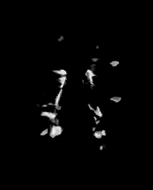
\includegraphics[height=4cm]{figures/lesions.png}};
\end{scope}

% 1-channel input

\foreach \x in {20} {
\begin{scope}[xshift=\x pt]
\draw[fill=white, fill opacity=0.75]
  (0,0) coordinate(A\x) -- ++(90:4) coordinate (B\x) -- ++(30:2) coordinate
  (C\x) -- ++(-90:4) coordinate (D\x) -- cycle;
  
\draw (0,3)
   ++(30:0.25) \ifnum\x=20 coordinate (a1) \else -- +(0:10pt) +(0:0) \fi
-- ++(90:0.5)  \ifnum\x=20 coordinate (b1) \else -- +(0:10pt) +(0:0) \fi
-- ++(30:0.25) \ifnum\x=20 coordinate (c1) \else -- +(0:10pt) +(0:0) \fi
-- ++(-90:0.5) \ifnum\x=20 coordinate (d1) \else -- +(0:10pt) +(0:0) \fi
-- ++(210:0.25);
\end{scope}
}

\node[pin=30:Visible\\ units] at ($(C20)!0.25!(D20)$) {};

% Transition

\draw ($(a1)!0.5!(c1)$) ++(55pt,-5pt) coordinate (e1);
\draw (a1) -- (e1);
\draw (b1) -- (e1);
\draw (c1) -- (e1);
\draw (d1) -- (e1);

% First layer hidden units

\foreach \x in {80,85,90,95,100,105} {
\begin{scope}[xshift=\x pt,yshift=1.5cm,scale=0.5]
\draw[fill=white, fill opacity=0.75]
  (0,0) coordinate(A\x) -- ++(90:4) coordinate (B\x) -- ++(30:2) coordinate
  (C\x) -- ++(-90:4) coordinate(D\x) -- cycle;
   
\draw (0,2.5)
   ++(30:0.25) \ifnum\x=105 coordinate (a2) \else -- +(0:10pt) +(0:0) \fi
-- ++(90:1)    \ifnum\x=105 coordinate (b2) \else -- +(0:10pt) +(0:0) \fi
-- ++(30:0.5)  \ifnum\x=105 coordinate (c2) \else -- +(0:10pt) +(0:0) \fi
-- ++(-90:1)   \ifnum\x=105 coordinate (d2) \else -- +(0:10pt) +(0:0) \fi
-- ++(210:0.5);
\end{scope}
}

\draw[decorate,decoration={brace,raise=4pt,mirror}]
%(A80) --node[below=8pt] {$N = 32$} (A80-|D105);
(A80) --node[below=8pt] {$N = 32$} (A80-|D105);

\draw ($(a2)!0.5!(c2)$) ++(0:38pt) coordinate (e2);
\draw (a2) -- (e2);
\draw (b2) -- (e2);
\draw (c2) -- (e2);
\draw (d2) -- (e2);

\node[pin=30:Hidden\\ units] at ($(C105)!0.2!(D105)$) {};

% Second layer hidden units

\foreach \x in {145, 150, ..., 175, 180} {
\begin{scope}[xshift=\x pt,yshift=2.25cm,scale=0.25]
\draw[fill=white, fill opacity=0.75]
  (0,0) coordinate(A\x) -- ++(90:4) coordinate (B\x) -- ++(30:2) coordinate
  (C\x) -- ++(-90:4) coordinate(D\x) -- cycle;
\draw (0,1.75)
   ++(30:0.25) \ifnum\x=180 coordinate (a3) \else -- +(0:20pt) +(0:0) \fi
-- ++(90:2)    \ifnum\x=180 coordinate (b3) \else -- +(0:20pt) +(0:0) \fi
-- ++(30:1)    \ifnum\x=180 coordinate (c3) \else -- +(0:20pt) +(0:0) \fi
-- ++(-90:2)   \ifnum\x=180 coordinate (d3) \else -- +(0:20pt) +(0:0) \fi
-- ++(210:1);
\end{scope}
}

\draw[decorate,decoration={brace,raise=4pt,mirror}]
(A145) --node[below=8pt] {$N = 64$} (A145-|D180);

\draw ($(a3)!0.5!(c3)$) ++(0:18pt) coordinate (e3);
\draw (a3) -- (e3);
\draw (b3) -- (e3);
\draw (c3) -- (e3);
\draw (d3) -- (e3);

% Third layer hidden units

\foreach \x in {200, 205, ..., 240} {
\begin{scope}[xshift=\x pt,yshift=2.625cm,scale=0.125]
\draw[fill=white, fill opacity=0.75]
  (0,0) coordinate(A\x) -- ++(90:4) coordinate (B\x) -- ++(30:2) coordinate
  (C\x) -- ++(-90:4) coordinate(D\x) -- cycle;
\end{scope}
}

%\node[rotate=90] at(270pt,2.75cm) {Serialize hidden units};

% Forth layer visible units (dense)

\begin{scope}[xshift=280pt, yshift=2.75cm]
\foreach \x/\y in {0/-2, 1/-1.5, 2/-1, 3/-0.5, 4/0, 5/0.5, 6/1, 7/1.5, 8/2} {
  \node[circle, draw] (V\x) at (0,\y) {};
}
\end{scope}

\draw[shorten >=10pt,shorten <=10pt,dashed] (A240)--(V0.south west);
\draw[shorten >=10pt,shorten <=10pt,dashed] (A240|-C240)--
%node[label=120:Vectorize\\ hidden units] {}
(V8.north west);

\draw[decorate,decoration={brace,raise=4pt,mirror}]
(A200) --node[below=8pt,fill=white] {$N = 32$} (A200-|D240);

%\node[rotate=90,fill=white,align=center] at(270pt,2.75cm) {Serialize\\ hidden
%units};

% Forth layer hidden units (dense)

\begin{scope}[xshift=320pt, yshift=2.75cm]
\foreach \x/\y in {0/-1, 1/-0.5, 2/0, 3/0.5, 4/1} {
  \node[circle, draw] (H\x) at (0,\y) {};
}
\end{scope}

\foreach \x in {0, ..., 8} {
  \foreach \y in {0, ..., 4} {
    \draw[very thin] (V\x)--(H\y);
  }
}

% Fifth layer hidden units (distribution parameters)

\begin{scope}[xshift=360pt, yshift=2.75cm]
\foreach \x/\y in {1/0.25, 2/-0.25} {
  \node[circle, draw, label=0:$L_\x$] (L\x) at (0,\y) {};
}
\end{scope}

\foreach \x in {0, ..., 4} {
  \foreach \y in {1,2} {
    \draw[very thin] (H\x)--(L\y);
  }
}
\end{scope}

%%%%%%%%%%%%%%
% Joint layer
%%%%%%%%%%%%%%

% yshift = 2.75 - 6/2 = -0.25

\begin{scope}[xshift=380pt, yshift=-0.25cm]
\foreach \x/\y in {1/-0.75, 2/-0.25, 3/0.25, 4/0.75} {
  \node[circle, draw, label=0:$J_\x$] (J\x) at (0,\y)
  {}; }
\end{scope}

\foreach \x in {0, ..., 4} {
  \foreach \y in {1, ..., 4} {
    \draw[very thin] (h\x)--(J\y);
    \draw[very thin] (H\x)--(J\y);
  }
}

\node[yshift=-15pt, fill=white, inner sep=3pt] at (h0) {$N = 16$};

\draw[decorate,decoration={brace,raise=30pt,mirror}] (V0.south-|J1)
--node[dbnlabel, below=35pt, sloped] {Joint DBN} (v8.north-|J1);

\end{tikzpicture}
%\end{center}
\end{headerblock}

%%%%%%%%%%%%%%%%%%%%%%%%%
% Evaluation
%%%%%%%%%%%%%%%%%%%%%%%%%

\begin{headerblock}{Evaluation}{row=0, column=2, span=2,
name=evaluation}

% \vspace{0.5em}

\minisection{Morphology, Lesion Distribution, and Joint Manifold}

\begin{compactitem}
\item From left to right, the images show slices from generated volumes from
the morphology, lesion, and joint model.
\item The morphology model captures ventricular enlargement ($D_1$)
and decrease in brain size ($D_2$) as the main modes of variation.
For the lesion model, $L_1$ captures an increase in lesion load throughout
the WM, while $L_2$ captures primarily periventricular lesion load variations.
The parameters of the joint model capture combinations of the variability
found in the individual models. 
\end{compactitem}
\begin{center}
\newlength{\subfigwidth}
\setlength{\subfigwidth}{0.232\textwidth}
\begin{tikzpicture}
\node[inner sep=0.5em] (manifold){
\includegraphics[width=\subfigwidth]{figures/warps_t1_dark}};

\draw[->] (manifold.south west)--node[below=0.4em,inner sep=0] {$D_1$}
(manifold.south east);
\draw[->] (manifold.south west)--node[above=0.4em,sloped,inner sep=0] {$D_2$}
(manifold.north west);

\end{tikzpicture}
\quad
\begin{tikzpicture}

\node[inner sep=0.5em]
(manifold){\includegraphics[width=\subfigwidth]{figures/p442_d0_full_h16-2}};

\draw[->] (manifold.south west)--node[below=0.4em,inner sep=0] {$L_1$}
(manifold.south east);
\draw[->] (manifold.south west)--node[above=0.4em,sloped,inner sep=0] {$L_2$}
(manifold.north west);

\end{tikzpicture}
\quad
\begin{tikzpicture}

\node[align=left,fill=black,inner sep = 0pt] (manifold1) {
  \mbox{}\\[2pt]
  \includegraphics[trim=0 340 0 0,clip,width=\subfigwidth]
    {figures/full_rl1_h4_sag}\\[8.5pt]
  \includegraphics[trim=0 0 0 150,clip,width=\subfigwidth]
    {figures/full_rl1_h4}
};
\node[fit=(manifold1),inner sep=0.5em] (manifold) { };

\foreach \x/\y in {0.125/1, 0.375/2, 0.625/3, 0.875/4} {
  \node[left,inner sep=0pt] at ($(manifold.north west)!\x!(manifold.south
  west)$) {$J_\y$}; }

\draw[->] (manifold.south west)--node[below=0.4em,inner sep=0] {$J_x$}
(manifold.south east);

\end{tikzpicture}
\end{center}

\minisection{Correlations with Clinical Scores}
\begin{compactitem}
\item Pearson correlations $r$ of clinical scores with distribution parameters
of the morphology model ($D_1$, $D_2$), lesion model ($L_1$, $L_2$), joint model
($J_1$, $J_2$, $J_3$, $J_4$), normalized brain volume (nBV), and lesion load
(LL). The level of statistical significance is indicated by the number of
asterisks (* $p < 0.05$, ** $p < 0.01$, *** $p < 0.001$).
\end{compactitem}
\begin{center}
\sisetup{
  round-mode = places,
  round-precision = 3,
  exponent-product = \cdot,
  detect-weight=true,
  detect-inline-weight=math,
  tight-spacing = false,
  table-align-text-post = false
}%

\def\tabspace{14pt}

\begin{tabular}{c@{\hspace{\tabspace}}c%
@{\hspace{\tabspace}}S[table-format=2.5]%
@{\hspace{\tabspace}}S[table-format=2.6]
@{\hspace{\tabspace}}S[table-format=2.6]
@{\hspace{\tabspace}}S[table-format=2.6]}
\toprule
 &  & {T25W} & {9-HPT} & {PASAT} & {MSFC} \\
 \midrule
 
\multirow{4}*{\minitab[c]{Individual\\ models}}
 & $D_1$ &
\bfseries -0.128976787246536** & -0.214588136146619*** & -0.282044527648157*** &
-0.314633263656368*** \\
 & $D_2$ & 0.0870255979372807 & 0.115835195120173* & 0.08923208653141 &
0.138616500875685** \\
& $L_1$ & -0.0581629511079419 & -0.231012897586838*** & -0.391822792658197*** &
-0.366992537420278*** \\
& $L_2$ & -0.091057480388512 & \bfseries -0.354478789398171*** &
\bfseries -0.426543205964196*** & \bfseries -0.463860459137063*** \\
\addlinespace
\multirow{4}*{\minitab[c]{Joint\\ model}}
 & $J_1$ & 0.107219513748914* & 0.285812780188632*** & 0.336253511146623*** &
0.378889115681159*** \\
 & $J_2$ & -0.037731447660239 & -0.209982769437628*** & -0.226800472678912***
& -0.255585426983655*** \\
& $J_3$ & \bfseries -0.117780586822506* & \bfseries -0.369169927947271*** &
\bfseries -0.452556545437486*** & \bfseries -0.494130959187706*** \\
& $J_4$ & -0.0491209563011896 & -0.205764640863705*** & -0.382954826511733*** &
-0.345529171963859*** \\
\addlinespace
\multirow{2}*{\minitab[c]{Imaging\\ biomarkers}}
 & nBV & 0.0530068558456253 & 0.143905618421747** & 0.246833144651129***
& 0.234774254053599*** \\
 & LL & -0.073681606595365 & \bfseries -0.286360084620956*** &
\bfseries -0.399646128024074*** & \bfseries -0.406222020153583*** \\
  
 \bottomrule
\end{tabular}
\end{center}

\minisection{Progression of a ``Mean'' SPMS Brain along a
Range of MSFC Scores}
\begin{compactitem}
\item Axial (top row) and mid-sagittal (bottom row) slices of volumes
representing the spectrum of MSFC scores from \num{1.5} to \num{-4.5}. A
decrease in MSFC shows the classic pattern of MS pathology.
\end{compactitem}
\begin{center}
\begin{tikzpicture}
\node[align=left,inner sep=0] (images) {
\includegraphics[width=0.4\textwidth]{figures/full_rl1_h4_MSFC_nolesion} \\
\includegraphics[width=0.4\textwidth]{figures/full_rl1_h4_MSFC_sag_nolesion}
};
\foreach \x/\y in {0.1/1.5, 0.3/0, 0.5/-1.5, 0.7/-3, 0.9/-4.5} {
  \node[above=0.4em] at ($(images.north west)!\x!(images.north east)$) {\y}; }
\end{tikzpicture}
\quad
\begin{tikzpicture}
\node[align=left,inner sep=0] (images) {
\includegraphics[width=0.4\textwidth]{figures/full_rl1_h4_MSFC} \\
\includegraphics[width=0.4\textwidth]{figures/full_rl1_h4_MSFC_sag}
};
\foreach \x/\y in {0.1/1.5, 0.3/0, 0.5/-1.5, 0.7/-3, 0.9/-4.5} {
  \node[above=0.4em] at ($(images.north west)!\x!(images.north east)$) {\y};
}
\end{tikzpicture}
\end{center}

\end{headerblock}

\begin{headerblock}{Conclusions}{below=evaluation, column=2,above=bottom}
\begin{compactitem} 
  \item Our model can automatically discover the classic patterns of MS
  pathology, as well as more subtle ones.
  %\item The parameters computed by our model have strong relationships to MS
  %clinical scores.
  \item The parameters of the joint model correlate stronger with MS clinical
  scores than the parameters of either individual model.
  \item The parameters of the individual models and the joint model correlate
  stronger with MS clinical scores than traditional imaging biomarkers.
\end{compactitem} 
\end{headerblock}

% \begin{headerblock}{Acknowledgement}{below=method, column=0, span=2
% %boxheaderheight=1.6em
% }
% This work was supported by the Natural Sciences and Engineering Research
% Council of Canada and the Milan and Maureen Ilich Foundation.
% \end{headerblock}

%\normalsize 
\begin{headerblock}{Contact Information}{below=evaluation, column=3,
above=bottom,
%boxheaderheight=1.6em
}
% \begin{tabular}{@{}c@{\, }ll}
\begin{tabular}{@{}cll}
  \Letter & \texttt{tombr@msmri.medicine.ubc.ca} \\
  \Mundus & \url{http://tbrosch.blogspot.com/} \\
  & \multicolumn{1}{c}{\includegraphics[width=0.5\textwidth]{figures/contact}}
\end{tabular}
%\Letter\ \texttt{tombr@msmri.medicine.ubc.ca}\quad\Mundus{}
%\url{http://tbrosch.blogspot.com/}
\end{headerblock}

% TODO: add references
% TODO: Put a picture of me on the poster so people can find me at the
% conference if I'm not at my poster

% \headerbox{Contact}{name=contact,below=acknowledge}{
% Please contact us via e-mail:
% \begin{compactitem}
%   \item Tom Brosch: \texttt{tombr@msmri.medicine.ubc.ca}
%   \item Roger Tam: \texttt{roger.tam@ubc.ca}
% \end{compactitem}
% }

\end{poster}

\end{document}